\section{Initial project plan}

TODO: write a few sentences to describe the GANTT diagram 

\begin{figure}[h!]
\centering
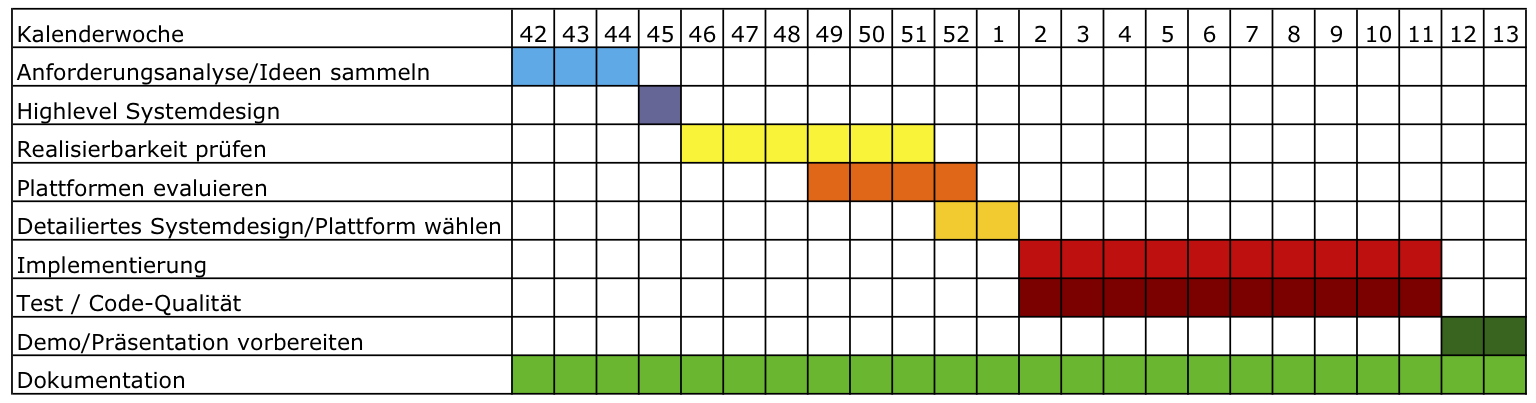
\includegraphics[width=16cm]{pics/gantt2.png}
\caption{Gantt diagram of the initial project plan (planing at project start)}
\label{gantt1}
\end{figure}

\section{Refined project plan}

TODO: insert second GANTT-diagram

TODO: extend task-list, introduce the list as milestones for second GANTT-diagram



\begin{itemize}
\item longer platform evaluation phase
\item added technology scouting phase for selected platform
\item add milestones in implementation phase
\end{itemize}
At the beginning of calendar week 7 it became obvious, that the number of open ToDos and the amount of time left until the project end after calendar week 13 required a more success-oriented development methodology.\\
For this purpose the development block (red in GANTT diagram) needs to be divided into smaller tasks or milestones, both for already completed work and for future tasks.\\

Up to this point, we were able to fulfill the following tasks:
\begin{itemize}
\item gather system requirements
\item define clean abstract system structur
\item choose appropriate OS and platform for the project
\item derive a OS specific system structure
\item install and get used to Android SDK
\item port Traveling Salesman routing engine to Android
\item solve biggest performance issues with routing engine
\item reverse-engineer the non-public Android calendar interface
\item finalize routing interface and implementation for Android
\item finalize calendar API
\item build system integration framework for Android OS, specifically  location and time triggered background tasks and user interaction
\item merge system parts into one unified application
\end{itemize}

 For the remaining 6 weeks of the project the following ToDos are left:
 \begin{itemize}
\item Determine performance of routing engine, identify bottlenecks and problems for future fixing
\item implement GUI for the task ''Generate and Manage Tasks''
\item implement GUI for the task ''Build and Manage day-plan''
\item implement background task ''optimize day-plan''
\item implement background task ''check day-plan for reachability of appointments''
\item write test-cases for the most important system parts (specifically the parts that could be reused in future projects)
\end{itemize}
